%%%%%%%%%%%%%%%%%%%% author.tex %%%%%%%%%%%%%%%%%%%%%%%%%%%%%%%%%%%
%
% sample root file for your "contribution" to a contributed volume
%
% Use this file as a template for your own input.
%
%%%%%%%%%%%%%%%% Springer %%%%%%%%%%%%%%%%%%%%%%%%%%%%%%%%%%


% RECOMMENDED %%%%%%%%%%%%%%%%%%%%%%%%%%%%%%%%%%%%%%%%%%%%%%%%%%%
\documentclass[graybox]{svmult}

% choose options for [] as required from the list
% in the Reference Guide

%\usepackage{mathptmx}       % selects Times Roman as basic font

\usepackage{helvet}         % selects Helvetica as sans-serif font
\usepackage{courier}        % selects Courier as typewriter font
\usepackage{type1cm}        % activate if the above 3 fonts are
                            % not available on your system
%
\usepackage{makeidx}         % allows index generation
\usepackage{graphicx}        % standard LaTeX graphics tool
                             % when including figure files
\usepackage{multicol}        % used for the two-column index
\usepackage[bottom]{footmisc}% places footnotes at page bottom

% see the list of further useful packages
% in the Reference Guide

\usepackage[T1]{fontenc}
\usepackage{ae,aecompl}
\usepackage{caption}
\usepackage{subcaption}

\usepackage{float}
\floatstyle{plaintop}
\restylefloat{table}

\widowpenalty=10000
\clubpenalty=10000
\setlength{\belowcaptionskip}{+0.3ex}
\setlength{\abovecaptionskip}{3pt plus 3pt minus 2pt}

\makeindex             % used for the subject index
                       % please use the style svind.ist with
                       % your makeindex program

%%%%%%%%%%%%%%%%%%%%%%%%%%%%%%%%%%%%%%%%%%%%%%%%%%%%%%%%%%%%%%%%%%%%%%%%%%%%%%%%%%%%%%%%%

\begin{document}

\title*{In-Situ Visualization in Fluid Mechanics using Open-Source tools: integration of Catalyst into Code\_Saturne}
% Use \titlerunning{Short Title} for an abbreviated version of
% your contribution title if the original one is too long
\author{Name of First Author and Name of Second Author}
% Use \authorrunning{Short Title} for an abbreviated version of
% your contribution title if the original one is too long
\institute{Name of First Author \at Name, Address of Institute, \email{name@email.address}
\and Name of Second Author \at Name, Address of Institute \email{name@email.address}}
%
% Use the package "url.sty" to avoid
% problems with special characters
% used in your e-mail or web address
%
\maketitle

\abstract{
The volume of data produced by numerical simulations performed on high
performance computers is becoming increasingly large. The visualization of
these large post-generated volumes of data is currently a bottleneck for the
realization of engineering and physics studies in industrial environments. In
this context, Catalyst is a prototype in-situ visualization library developed by
Kitware to help reduce the data post-treatment overhead. On the other side,
\CS is a Computational Fluid Dynamics code used at EDF, one of the
biggest electricity producers in Europe, for its large scale simulations. Both
Catalyst and \CS are Open Source software. In this
chapter we present a study case where Catalyst is integrated into \CS. We
evaluate the feasibility and performance of this integration by running several
use cases in one of our corporate supercomputers.
} % end of abstract



\section{Introduction}
Computational Fluid Dynamics (CFD) is a fundamental step for the study and
optimization of electricity production. Indeed, current power plants use water
as a mean of convective heat transfer. Consequently, the simulation and
visualization of fluid dynamics phenomena is of great importance for the energy
industry. Electricité de France (EDF), one of the largest electricity producer in Europe, has
been developing for the past 15 years an open source CFD code named \CS. \CS performs
CFD computations on very large models~\cite{5644955}. EDF owns
several supercomputers that regularly run this code in order to perform CFD
analysis involving large amounts of data. In this context, the post-processing
and visualization steps become critical. 
%% =======

EDF also develops, in collaboration with OpenCascade and the French Center of
Atomic Research (CEA), an open-source numerical simulation platform called
SALOME. This platform provides generic methods for pre- and post-processing of
numerical simulations. SALOME is based on an open architecture made of reusable
components such as computer-aided design (CAD),
meshing, high performance computing (HPC) execution management, multi-physics coupling, data post-processing
and visualization. The visualization module of the SALOME platform is currently based
on the open-source post-processing platform ParaView. Furthermore, \CS is often used 
in conjunction with the the SALOME platform.

In the past, studies and improvements in scientific simulation have been mainly
focused on the solver, due to being the most cycle-consuming part in the
simulation process. Thus, visualization has been traditionally run sequentially
on a smaller computer and at the very end of the solver computation. At the
time, this was easily explained by the small need for both memory and
computation resources in most of the visualization cases. Nevertheless, with the
increase of our computational capabilities, we tend to use and generate much
more data than what we were used to. Thus, as the scale of CFD simulation
problems is getting wider, specific issues are emerging related to input/output
efficiency. In particular, data generated during the solver computation and
used for the visualization are the source of a worrisome overhead. Even worse,
some researchers are starting to spend more time writing and reading data
than actually running solvers and visualizations~\cite{1742-6596-125-1-012099}.
%Sometimes referred as Big Data, 
This new trend compels us to design new input/output (I/O) strategies and consider
visualization as a part of our high-performance simulation systems.

For some years, $in$-$situ$ visualisation techniques have been successfully 
applied in different contexts and mainly by research institutes. 
In this chapter, we present an overview of the efforts 
needed to transition a traditional simulation code to an $in$-$situ$ model 
in an industrial environment. This is the reason why care have been taken 
constructing uses cases that are representative of our current visualisation problems. 

Most fluid dynamic engineers at EDF R\&D are currently visualizing lower temporal and spatial 
resolution versions of their simulations in order to avoid I/O bottlenecks when large quantities of data are involved.
We decided to address the subject of co-processing and $in$-$situ$
visualization which has been proved to be an effective solution against the current
limitations of this problem~\cite{sandiareport}, \cite{4090186}. Our aim is to provide 
EDF engineers with an operational research-oriented tool in a mid-term basis.
%Moreover, while visualization has been traditionnally performed on smaller
%computer, studies show that visualization algorithms can often be run
%efficiently on recent supercomputers~\cite{4090186}. 
For this, we chose to evaluate Catalyst as an industrial tool for performing
$in$-$situ$ visualization. 
Catalyst is a library, developed by Kitware, which implements the
co-processing for ParaView by defining the visualization process through the ParaView user 
interface and exploiting VTK's parallel algorithms for the post-processing of data 
generated by numerical simulation~\cite{6092322}. 

In this chapter, we report a study upon the effectiveness and scalability of a
prototype implementation of the co-processing in an industrial case based on the
coupling of \CS with Catalyst. In section~\ref{sec:related} we
discuss related work on recent visualization $in$-$situ$ systems. We then
introduce, in section~\ref{sec:cs} \CS, the CFD code developed at EDF
R\&D. In section ~\ref{sec:catalyst} we present our integration of Catalyst into
\CS and how the system is used by EDF users in the context of fluid dynamic
simulations. Section~\ref{sec:results} describes our use case and presents
results on one of our corporate clusters. Finally, section~\ref{sec:conclusion} 
presents our analysis of the results and describes our ongoing and future work.


\section{Related Work}
\label{sec:related}

The size of generated data has become an important subject in high performance 
computing, due to the need of a better I/O efficiency in our computing 
system. To answer this problem, several visualization systems have been created.
We can distinguish two main approaches in recent solutions. The first one is to 
integrate a specific $in$-$situ$ visualization directly to the simulation code. 
Such approach proved to be an efficient way to provide co-processing for a given
simulation as well as a visualization system as it is the case in the hurricane
prediction~\cite{4015457} and earthquake simulation~\cite{4090186} systems.
This method has been proven to lead to good performances but is limited 
to a specific implementation.

The second approach is to provide a general post-processing framework letting the
simulation and the visualization code communicate together. EPSN which is a
general coupling system, allows for the connection of M simulation nodes to N
visualization nodes through a network~\cite{4020782}. This solution is a
loosely coupled approach, requiring separate resources and data transfer
through the network. This approach presents the advantage of not overloading
the nodes used for computation. Thus the visualization code does not interfere
with the execution of the simulation. Based on the same approach, a ParaView
plug-in named ICARUS~\cite{6152102} has been developed. 
It differs from EPSN in design by having lower requirements as it only needs
the use of a single HDF5 library and file driver extension. Such solutions
offer tools for researchers to interact with their simulations by allowing
them, not only to monitor their current states but also to modify
the parameters of the remaining simulation steps. Those computational steering
solutions as well as the RealityGrid
project~\cite{Harting03computationalsteering} focus on interactivity with
simulation whereas our main objective is to provide $in$-$situ$ visualization
operations to researchers while minimizing I/O overhead and disk
space use. 

Both built upon the well known parallel visualization library VTK, 
the application frameworks VisIt~\cite{1532795} and ParaView~\cite{964413} both provide through
the possibility to co-process simulation data via libsim~\cite{2386230} and Catalyst~\cite{6092322} respectively.  
Those $in$-$situ$ solutions are tightly coupled and while they
limit potential interactions with the running simulation, they also highly
reduce the need of network data transfer. Thus, they contribute to circumventing
the inefficiency of high performance computing I/O systems.
Those solutions take their benefits from directly accessing the simulation memory to
perform visualization tasks by simply asking for a pointer to the available
data. One major drawback of this approach is the necessity to provide a coherent data 
layout to those libraries. Moreover, as this type of
solution often gains from computing pre-determined visualization tasks, it is
not well suited for results exploration.  As building a steering solution for Code\_Saturne is out of
the scope of this case study, we do not consider these drawbacks as a limitation. 

After evaluating the performance solutions offered by ParaView and VTK, we choose Catalyst as 
our co-processing library for our case study as it answers EDF's visualization 
needs while focusing on the  reduce of data amount use. %Further, Kitware is still actively developing 
%Catalyst, and we are optimistic that more services allowing the interactions
%with the running simulation will soon be available.
Further, Kitware recently included services allowing the interactions with the
running simulation, the so-called Live Catalyst.



\section{\CS: A Computational Fluid Dynamics code}
\label{sec:cs}
\CS is a computational fluid dynamics software designed to solve the
Navier-Stokes equations in the cases of 2D, 2D axisymmetric or 3D
flows. Development started in 1997, with a first release in 2000, and the
code has been released as free software under a GPL licence since 2007.
Its main module is designed for the simulation of flows which may be
steady or unsteady, laminar or turbulent, incompressible or potentially
dilatable, isothermal or not. Scalars and turbulent fluctuations of scalars can
be taken into account. The code includes specific modules, referred to as
``specific physical models'', for the treatment of atmospheric flows, Lagrangian particle
tracking, semi-transparent radiative transfer, gas combustion, pulverised coal
combustion, electricity effects (Joule effect and electric arcs) and
compressible flows. \CS relies on a finite volume discretisation and
allows the use of various mesh types which may be hybrid (containing several
kinds of elements) and may have structural non-conformities (hanging nodes). The
parallelization is based on standard spatial partitioning with ghost cells
that facilitate data passing between adjacent cells lying across the boundaries
of disconnected parts using the Message Passing Interface. More
technical details are presented in~\cite{cs2004} and ~\cite{userguide},
and many resources are available at \url{http://www.code-saturne.org}.
\CS is also used as a base for the NEPTUNE\_CFD code, specialized in
multiphase flows, and which uses a different time stepping scheme,
but mostly the same volume discretization scheme.

As \CS is used for industrial cases involving complex flows, with turbulence
modeling requiring sufficiently fine resolution, large meshes are often
needed. In 2000, the largest meshes used for actual studies were around
1.5 million cells; today, they have reached up to 350 million cells.
More common studies use meshes about 10 times smaller than that.
Meshes up to 3.2 billion cells have been tested for a few time steps, to
ensure the code's internal mechanisms work well at scale.

\CS focuses on the solver, and its uses requires external tools for the
major part of the meshing and visualisation tasks, though the code itself offers
major preprocessing features to make these easier, such as parallel joining
of independently-built and read submeshes (whether conforming or not),
and user-definable postprocessing functions. Many input mesh and visualisation
output formats are supported (including the EDF and CEA MED format,
and the standardized CGNS format).

~\
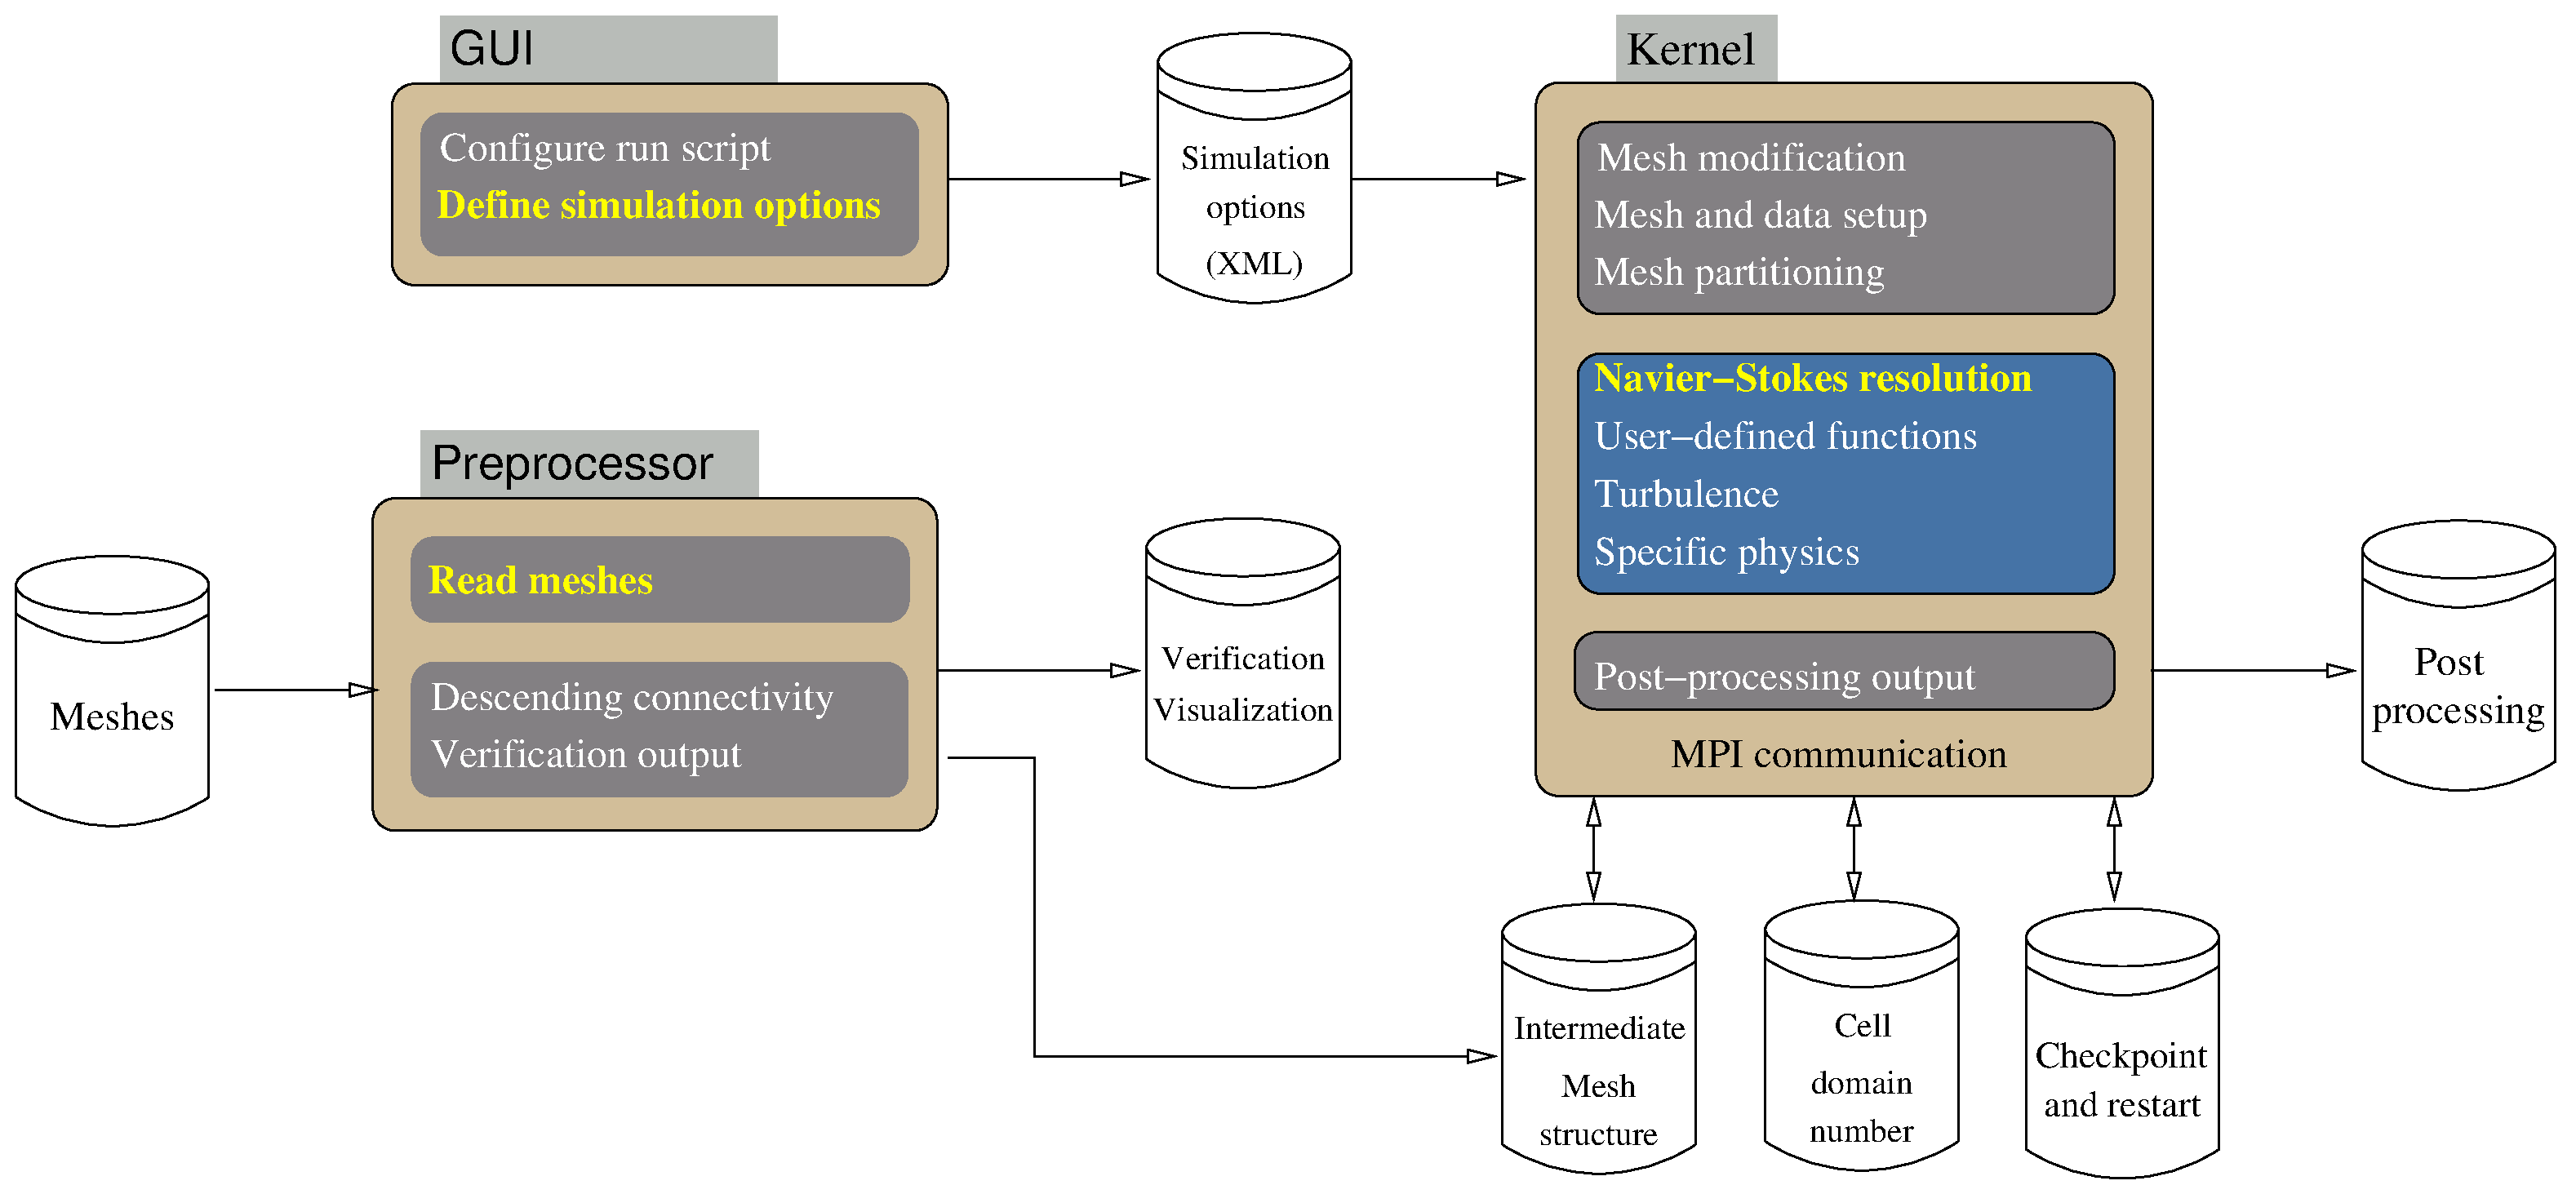
\includegraphics[scale=0.2]{pictures/cs_components.eps}
\captionof{figure}{\CS toolchain components.}
\label{fig:cs_components}
\vspace{+0.04in}
~\

The number of separate executable tools is quite reduced, with a few
interactive tools and associated commands designed for data setup.

To make the use of HPC as seamless as possible, without multiplying the
number of tools or requiring complex libraries or dependencies,
mesh, checkpoint/restart, and postprocessing output files
are partitioned independently: in addition to the connectivity of each
local mesh, which is described with a local numbering, global ids are also
maintained, for import and export purposes, and for ghost cell to
local cell matching. Multiple ranks participate in reading and writing
files using MPI-IO.

Typically, computational resource requirements are primarily determined
either by the time to solution, or the size of the model. For time to
solution, the number of cores may be selected in order to solve the problem
in a given time. In practice, optimal performance is often obtained
in a range of 30~000 to 60~000 cells per rank on a typical HPC cluster
(this being the best compromise between communication latency and
cache behavior). On machines with very good network/compute performance
ratios, such as IBM Blue Genes or Cray X series, this range may be
a bit wider.


\section{Using Catalyst}
\label{sec:catalyst}

Catalyst is the coprocessing library of ParaView. 
It has been designed to be tightly coupled with simulation codes to perform in situ analysis at run time. 
Catalyst leverages the Visualization Toolkit (VTK) for scalable data analysis and visualization. Furthermore, it can be coupled with the ParaView In Situ Analysis framework to perform run-time visualization of data extracts and steering of the data analysis pipeline.
Catalyst provides two sets of tools: one for simulation users and one for simulation developers.

For simulation users, it is possible to create a coprocessing pipeline using two different methods. 
The first method does not require any knowledge of ParaView and relies on pre-generated scripts. These predefined scripts can be written in C++ or Python and are, usually, expected to run without any configuration options. 
The second method uses the ParaView interface to generate a coprocessing script
from scratch and intuitively adjust its parameters as needed. This method is
similar to using ParaView interactively to setup desired post-processing
pipelines. The goal of these pipelines is to extract post-processed information
during the simulation run. Ideally one should start with a representative
dataset from the simulation. It is also possible to modify directly the
generated Python's scripts which have been previously created using ParaView.
However, this would require a knowledge of the ParaView Python application
programming interface (API).

For simulation developers, Catalyst provides the tools to create an adaptor between the simulation code and the visualization pipeline.
The adaptor binds the simulation code and Catalyst so that both the functions of the simulation code and the general-purpose API of Catalyst can be accessed. As Catalyst itself is independent of the simulation code, only the adaptor has to be developed by the designers of the solver. This flexibility is critical in order to successfully integrate external code into complex simulations usually running with different languages and packages. Catalyst is also easily extensible so that users can deploy new analysis and visualization techniques to existing coprocessing installations. Catalyst provides all the communication and synchronization routine and the pipeline mechanics necessary for coprocessing. Catalyst also provides powerful data processing capabilities through VTK filters as well as many writers and support for compositing and rendering.

The Catalyst library has also been developed with features to address limitations that come with pre-configuring a pipeline, but there may still be some unexpected data in the arbitrary simulation. To address these situations, the pipeline must be adjusted interactively.
The Catalyst library can leverage ParaView's client server mechanism to allow an
interactive ParaView client to connect to a server running inside an in situ
pipeline. ParaView can then read from a Catalyst data source like it reads from
a file. This enables construction/modification of a pipeline interactively in the ParaView client via this live data source. Additionally, by enabling the client-server architecture in the Catalyst library, some or all of the data analysis and visualization pipeline can offload, if desired, to a separate machine, e.g., a smaller visualization cluster with specialized graphics hardware.

\vspace{+0.25in}
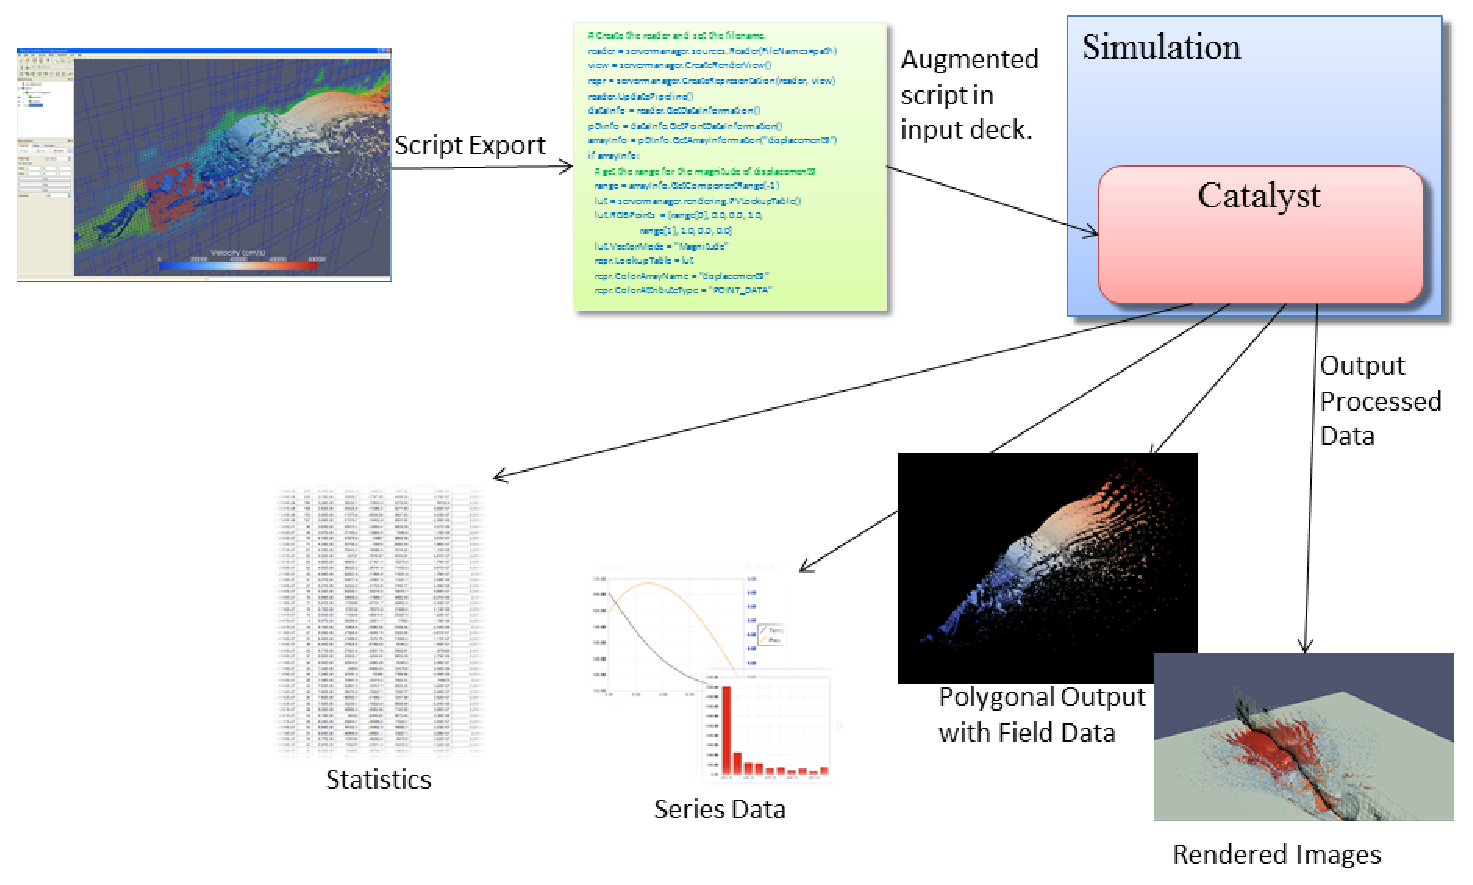
\includegraphics[scale=0.47]{pictures/CatalystFullWorkFlow.eps}
\captionof{figure}{Overall Catalyst workflow.}
\label{fig:catalyst}
\vspace{-0.14in}

\subsection{\CS with Catalyst}

Using Catalyst with \CS is quite straightforward, and fits
quite naturally in the existing architecture. In this section we describe first
how we implemented an adaptor for Catalyst and then we present how we configured the
post-processing pipeline.

\subsubsection{Adaptor implementation}
When embedding Catalyst there is always a non-zero cost in terms of time, memory and number of processors. 
Naively, one could simply
address these issues by requesting a greater number of processors, but in most cases this is
not possible nor practical. Therefore, great care must be taken in the implementation of the adaptors.
If memory is limited, the adaptor either uses complicated pointer manipulation or uses a smaller region
of memory. If memory is not limited, then deep copy of the simulation data structures into a VTK
data object doubles the resident memory, and also creates a CPU cost involved with copying the data.
The overriding overhead issue in embedding ParaView Catalyst in a simulation code is the memory
management in an adaptor translating data structures in the running simulation.

In order to co-process the simulation data, Catalyst must be provided with the
data formatted to the VTK data object structure. To accomplish this task, several
solutions are possible, depending on the format used for the data
of the simulation code. In the case where the format of the simulation code is
similar to VTK  and, moreover, the simulation data can be shared at any time,
then it is possible to feed Catalyst with a direct pointer to the simulation
memory. This option is indeed preferred, when possible, as it allows to decrease the memory footprint.
Another option is to fully or partially copy the data from the
simulation into a VTK object, and then send this object to Catalyst.

As users of \CS are provided with several output formats and as the data
structure in our simulation differs from the VTK data object structure, feeding
Catalyst with a direct pointer to the simulation memory is not possible. Thus, in this configuration
data is copied from the simulation into a VTK data object. In fact, we
 allocate a vtkDoubleArray data structure to store our data for Catalyst. Furthermore, we
provide a pointer of this VTK data structure to \CS so it can transform
its simulation data and then fill the VTK data object.

The memory cost increase of our solution can be alleviated by using more
machines. The CPU cost of the copy is in a range similar to the one needed when
adapting simulation data to a specific output format. This cost is largely
affordable comparatively to the time to write data to disk when storing time
step specific outputs. 

\subsubsection{Pipeline configuration}
\label{sec:pip_conf_tools}

From the point of view of an engineer performing a fluid mechanics simulation
using \CS, the workflow of a co-processing simulation is 1) to define
a ParaView pipeline describing what the user wants to study and 2) to run the
simulation. Since users are already familiar with fluid mechanics
simulations, defining the pipeline for the co-processing remains the main
sticking point. Thus this new process should be done in an efficient way and 
should not become a cumbersome bottleneck. This point is of great importance, especially in
an industrial environment like ours.

As we have explained in the previous section, the definition of a Catalyst pipeline can be achieve either 
programmatically or via the ParaView interface. In our industrial context, the former 
was considered too complicated and time consuming for the end user, especially when setting camera
parameters is needed, as no visualization feedback is provided. Therefore, the Catalyst pipeline has 
been created using the ParaView user's interface. This solution appears to be much easier as one
can interact with ParaView in the same way he/she uses to when
visualizing the results a posteriori. This solution is also easier to deploy with ParaView using 
its companion co-processing plugin. 

Indeed, using ParaView to define the co-processing requires a representative input dataset.
One could use the available resources on a large cluster in order to setup the pipeline. However we chose to  
provide a simplified or under-sampled version of the large geometry to define the
pipeline. In fact, this strategy is possible in ParaView but some
characteristics of the initial geometry must be present in its simplified version; more importantly the name of the data fields must
remain the same, as they are part of the definition of the pipeline.

The generation of the co-processing pipeline implies several steps.
First of all, the users start with a Computer Aided Design (CAD)
version of the geometry which is parametrized. This parametric representation
can generate meshes at different resolution levels. In our case, this is
performed inside the open-source SALOME~\cite{4291178} platform for numerical simulation. 

We then generate two different meshes, one at high resolution (up to 204M
hexahedrals in the current use cases) that will be used for the CFD
simulation and one with a lower resolution to define the pipeline (700 000
hexahedrals in our use cases). The lowest resolution mesh is fed into \CS to perform a short
simulation. This allows ParaView to obtain a representation containing not
only the geometry but also the result fields. This is the data that is then used to define the pipeline.
The different processing pipelines are presented next.


\section{Results}
\label{sec:results}

\subsection{Required User Interactions for Coprocessing}
   
\begin{figure}
  \centering
  \begin{subfigure}[b]{0.45\textwidth}
    \includegraphics[scale=0.195]{pictures/pieceofcake.eps}
    %\captionof{figure}{Original geometry for our use case}
    \captionof{figure}{}
    \label{fig:piece}
  \end{subfigure}
  ~
  \begin{subfigure}[b]{0.45\textwidth}
    \includegraphics[scale=0.41]{pictures/res.eps}
    %\captionof{figure}{A final coprocessed picture of our simulation. The simulation was run with 128 layers.}
    %\captionof{figure}{A final coprocessed picture of our simulation.}
    \captionof{figure}{}
    \label{fig:res}
  \end{subfigure}
  \caption{(a) original geometry of our use case\\
  \hspace{8em}(b)  a final coprocessed picture of our simulation}
\end{figure}

Before presenting our results we briefly describe how the user interactions was
performed. The following steps were necessary in order to use the developed
coprocessing technology:


1) The user generates a ``light version'' of the mesh. This step has already been
discussed in section~\ref{sec:pip_conf_tools}. Indeed, the user possess a CAD (Computer Aided
Design) version of the geometry that is parametrized, it is then possible to
obtain meshes at different spatial resolutions. A ``light mesh'' of small size in
memory and representative of the CAD geometry is obtained. Figure~\ref{fig:piece} represents
the ``light version'' of the mesh used in our experiments.


2) We run a short simulation (normally just a few seconds on a local machine) on the ``light mesh''.
This obtains the informations about the result fields we need to create a
visualisation pipeline in ParaView (e.g. temperature, pressure, velocity). We
could then say that we obtain an ``augmented light mesh''.


3) The mesh and the fields obtained at the end of step 2 are read in ParaView
and the user can define her/his visualisation pipeline. At the end of this step
a simple click in the ParaView interface will create a Python file that
programmatically defines the visualisation operations that will be performed
$in$-$situ$.


4) Finally the real simulation is ran using a full resolution size mesh. The
coprocessing part of the simulation reads the python script containing the
definition of the visualisation pipeline. This step is expected to be
time-consuming.
%, in our environment normally perform during several days in a
%supercomputer.

\subsection{Use Cases}

Our simulations have been run on Ivanoe, an EDF corporate supercomputer,
composed of 1382 nodes, each node having 12 cores for a total of 16584 cores. In
these simulations we associate one process by core and we use from 720 cores up
to 3600 cores. We include two use cases that were run on this supercomputer. The
choice of the cases is motivated by two main factors: the size of the mesh and
the complexity of the visualization pipeline. Let us define in more detail why
these two factors:

1) Mesh size. We chose to use two meshes representing the same geometry but at
different resolutions, one made of 51M hexahedral elements and another of 204M
hexahedrals. In our industrial environment at EDF most simulation engineers use
meshes composed by less than 51M of element, then we choose this mesh size to be
representative of the work performed by an average engineer in his work routine.
Furthermore, a 51M elements mesh more than doubles the size used in the results
presented in~\cite{6092322} for the PHASTA adaptor. On the other side, when researcher
oriented simulations are performed at EDF, they currently contain around 200M
elements. We choose then this size as a research oriented or ``heavy mesh'' kind
of simulation.

2) Pipeline complexity. We define two pipelines aimed to be representative of two
different situations: users just performing simple and light visualization
operations (mainly some slices in a volume) and another using very
time-consuming visualization tasks (mainly performing a volume rendering).

\begin{table}
\centering
\begin{tabular}{|p{1.5cm}|p{3.0cm}|p{2.70cm}|p{1.50cm}|}
\hline
\multicolumn{4}{|c|}{\textbf{USE CASES SUM UP}}\\
\hline
NAME & SIZE & PIPELINE & FIGURES \\
\hline
 %& & & \\
$CASE$\_$A$ & 51M hexahedrals, \newline industrial size case & \textbf{heavy}:
\newline volume rendering, \newline celldatatopointdata \newline and glyphs  &
5a 5c 5e\\
\hline
 %& & & \\
$CASE$\_$B$ & 204M hexahedrals, \newline research size case & \textbf{light}:
\newline 9 slices,\newline celldatatopointdata  & 5b 5d 5f   \\
\hline
\end{tabular}
%\vspace{-0.1in}
\caption{Description of our two use cases.}
\label{fig:tab}
%\end{figure}
\vspace{-0.15in}
\end{table}
In the following we name our uses cases:
$CASE$\_$A$, use case using an average mesh size of 51M hexahedrals and a
visualization pipeline including volume rendering which aims to be very time-consuming.
$CASE$\_$B$, our second use case, contains a light visualization pipeline simply
performing some slices but on a large mesh of 204M hexahedrals.

Table~\ref{fig:tab} summarizes the composition of these use cases. In all our use cases we
run a simulation consisting in a fluid with physical properties identical to
water passing through the mesh. Then the output is generated at each step, for a
total of 10 coprocessed visualization images.

%\vspace{-0.10in}
\subsection{Results}

\begin{figure}
        \begin{subfigure}[b]{0.50\textwidth}
          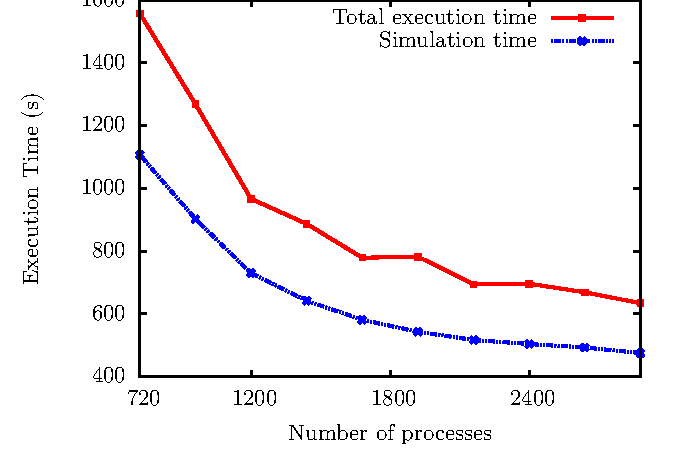
\includegraphics[scale=0.50]{pictures/test1.ps}
                \caption{Execution time with/out coprocessing}
                \label{fig:copro}
        \end{subfigure}%
        ~
        \begin{subfigure}[b]{0.50\textwidth}
          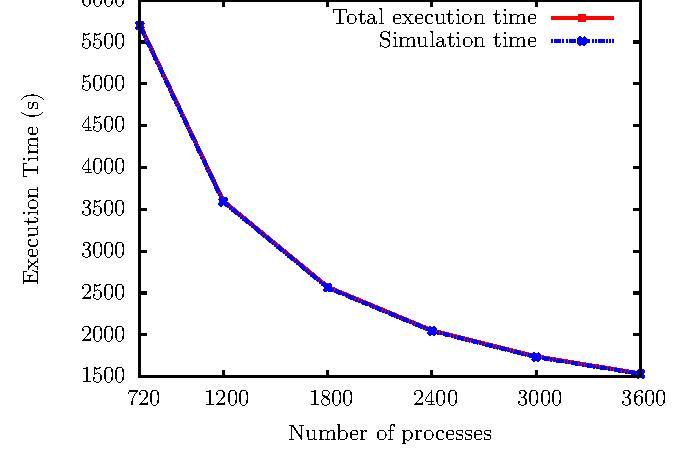
\includegraphics[scale=0.50]{pictures/test12.ps}
                \caption{Execution time with/out coprocessing}
                \label{fig:204copro}
        \end{subfigure}%

        \begin{subfigure}[b]{0.50\textwidth}
                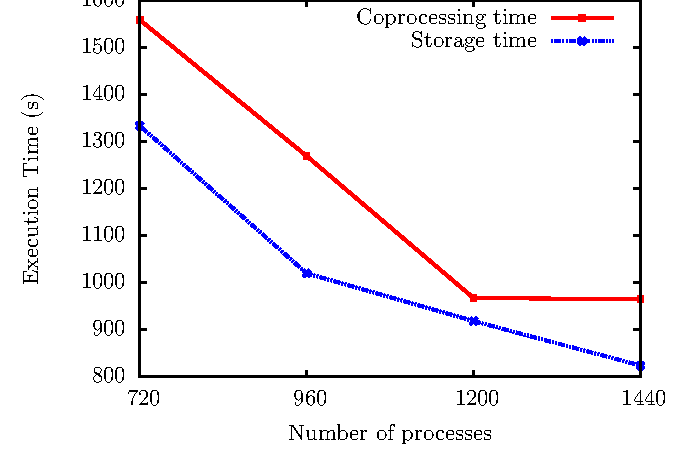
\includegraphics[scale=0.50]{pictures/test2.ps}
                \caption{Execution time comparison with storage.}
                \label{fig:ensight}
        \end{subfigure}
        ~
        \begin{subfigure}[b]{0.50\textwidth}
                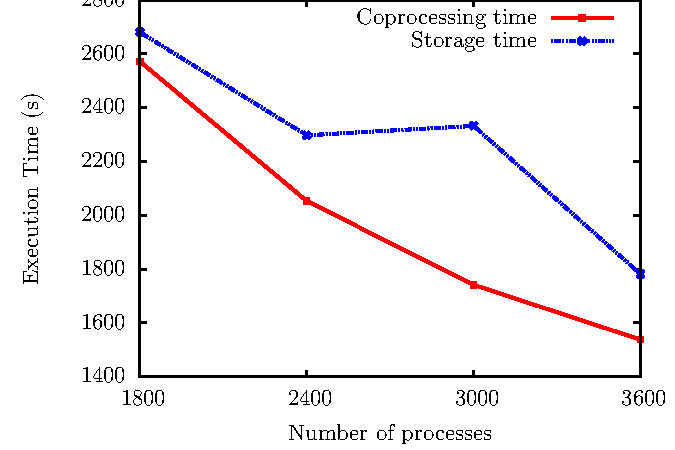
\includegraphics[scale=0.50]{pictures/test22.ps}
                \caption{Execution time comparison with storage.}
                \label{fig:204ensight}
        \end{subfigure}

        \begin{subfigure}[b]{0.50\textwidth}
                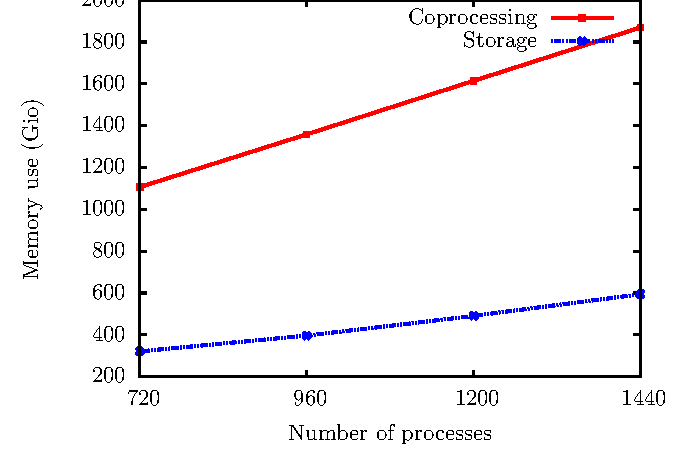
\includegraphics[scale=0.50]{pictures/test3.ps}
                \caption{Memory usage comparison with storage}
                \label{fig:mem}
        \end{subfigure}
        ~
        \begin{subfigure}[b]{0.50\textwidth}
                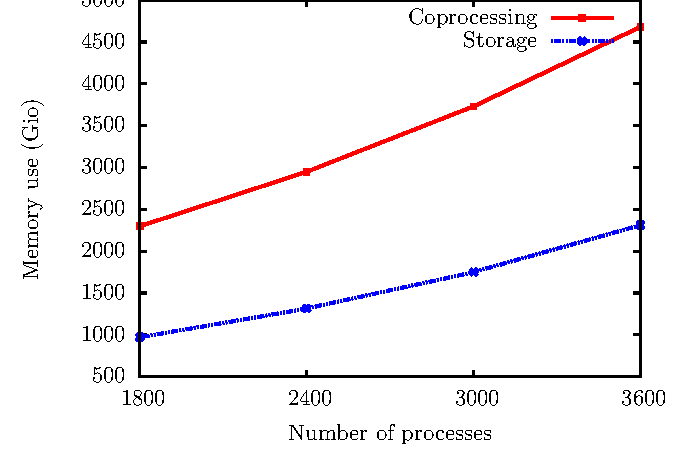
\includegraphics[scale=0.50]{pictures/test32.ps}
                \caption{Memory usage comparison with storage}
                \label{fig:204mem}
        \end{subfigure}
        \caption{CASE\_A (left) and CASE\_B (right) results}\label{fig:animals}
\end{figure}

Figure~\ref{fig:res} presents an image obtained from one of our $in$-$situ$
simulations with $CASE$\_$A$.
We see the flux of water moving around the vertical cylinders, the glyphs being attached 
to the velocity vectorial field. The color of the volume rendering represents 
the turbulent viscosity of the fluid. Figure~\ref{fig:copro} shows two graphs of
$CASE$\_$A$: in red the execution 
time versus the number of cores, in blue the execution time without
the coprocessing overload. We are satisfied by this overload that is contained
between 20 and 30\% of the total execution time. 
It looks like this overload is reducing with the increase in number of cores. 
Figure~\ref{fig:204copro} shows the exact same behavior but with $CASE$\_$B$. Both
graphs are difficult to distinguish as the time needed for coprocessing is
circumscribed between 6 and 10 seconds, the overload is lesser than one
percent of the total execution time.

We also decided to compare the Catalyst overhead with a non VTK based 
storage strategy that performs no visualization operations. Figure~\ref{fig:ensight} and~\ref{fig:204ensight}, 
show the comparison of the global execution time with Catalyst coprocessing
versus the simple Ensight Gold format storage. Figure~\ref{fig:ensight} presents
our implementation results with $CASE$\_$A$. This compares positively for Catalyst as the overhead
is approximately 10\% and looks decreasing when the number of cores increase.
Figure~\ref{fig:204ensight} presents our results for $CASE$\_$B$. Here we can see the potential of Catalyst when 
lighter and more relevant visualization tasks are processed. Indeed, there is no more 
overhead as we gain an average of 10\% of execution time while freeing
ourselves from storage issues (indeed, we evaluate the execution time peak of
3000 processes as a result of concurrent accesses on our 
supercomputer storage
disks). To emphasize this, table~\ref{fig:size_tab} shows how much data each
solution generates, namely a basic storage in Ensight Gold format versus our
coprocessing implementation using Catalyst. These informations are those of our
CASE\_B when performing a 10 steps simulation. Both size are
expected to grow proportionally to the size of the mesh input, and the number of
steps. Therefore, we expect the gain provided by the use of coprocessing 
to be
increasingly interesting when moving forward in use case size.

Finally, we also show the total memory use when running $in$-$situ$ visualization
compared to writing simulation results in Ensight Gold format in
figure~\ref{fig:mem} and~\ref{fig:204mem}. We observe that memory consumption
is increased by an approximate factor varying from 2 to 3. This can be
explained by both our first naive memory management approach and also by a
natural increase in memory consumption when visualization operations are to be
performed. Indeed, our memory management implies a consumption increased by more
than 2,
as we need to translate data for Catalyst but still need the former data to
pursue our simulation. Finally it may also be taken into account the actual memory consumption of the
chosen visualization tasks. 
%\begin{figure}[!h]
\begin{table}[!h]
\centering
\begin{tabular}{|p{3.5cm}|p{3.5cm}|}
\hline
\multicolumn{2}{|c|}{\textbf{*PROCESSING SIZE COMPARISON}}\\
\hline
STORAGE & COPROCESSING \\
\hline 
 %& \\
57Gio & 1,3Mio \\
\hline 
\end{tabular} 
%\vspace{-0.1in}
\caption{CASE\_B comparison between the size of processed results and simple storage. The simulation was run on 10 steps, with 10
pictures coprocessed.}
\label{fig:size_tab}
%\end{figure}
\end{table}


%\vspace{+0.04in}
%~\

%\clearpage
%\begin{minipage}[t]{\textwidth}
%\begin{minipage}{0.45\linewidth}
%\includegraphics[width=\linewidth]{/home/C26973/res.eps}
%\hspace{0.45in}
%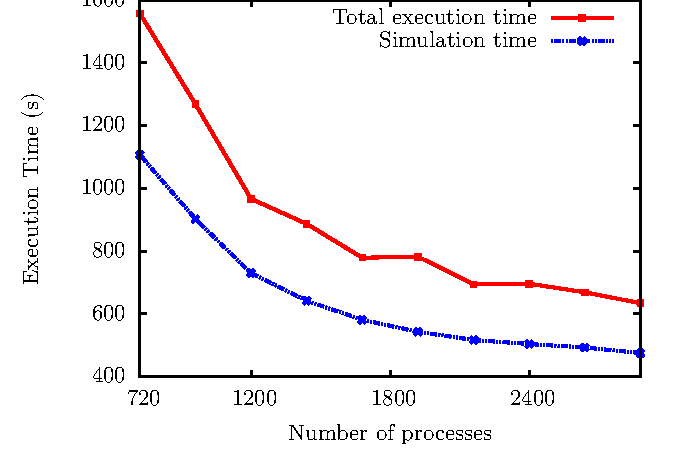
\includegraphics[scale=0.65]{pictures/test1.ps}
%\captionof{figure}{CASE\_A total execution time with and without the coprocessing.}
%\label{fig:copro}
%\vspace{+0.04in}
%~\
%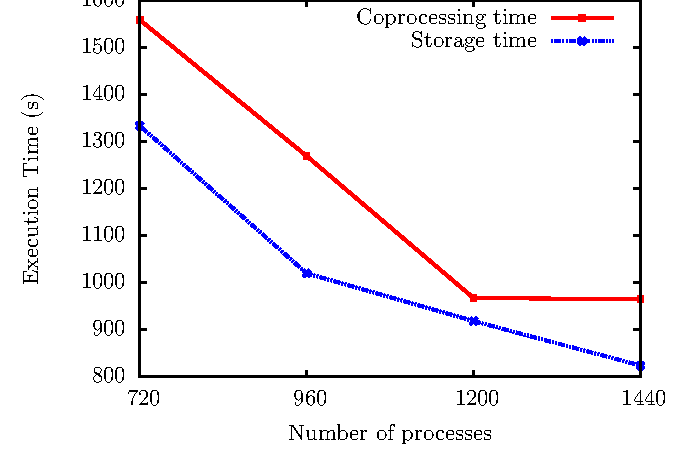
\includegraphics[scale=0.65]{pictures/test2.ps}
%\captionof{figure}{CASE\_A total execution time when using coprocessing and storage in
%Ensight Gold format.}
%\label{fig:ensight}
%\vspace{+0.04in}
%~\
%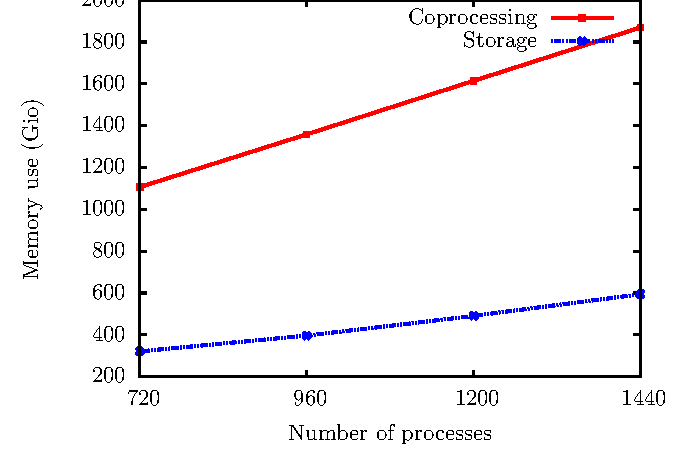
\includegraphics[scale=0.65]{pictures/test3.ps}
%\captionof{figure}{CASE\_A total memory usage when using coprocessing and storage in
%Ensight Gold format.}
%\label{fig:mem}
%\end{minipage}
%\hspace{0.05\linewidth}
%\begin{minipage}{0.45\linewidth}
%\includegraphics[width=\linewidth]{/home/C26973/pieceofcake.eps}
%\hspace{0.65in}
%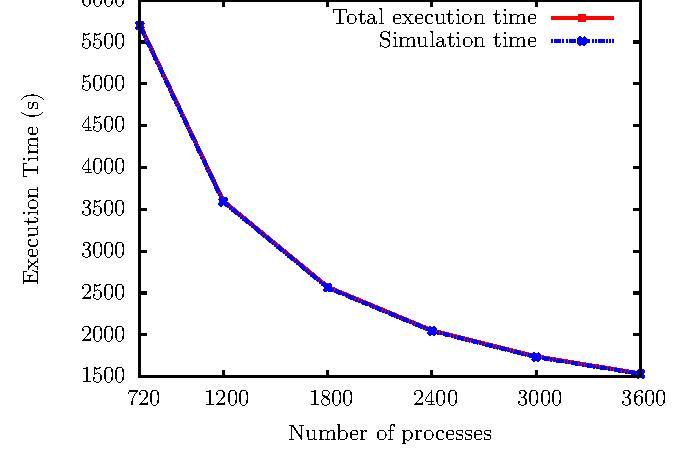
\includegraphics[scale=0.65]{pictures/test12.ps}
%\captionof{figure}{CASE\_B total execution time with and without the coprocessing.}
%\label{fig:204copro}
%\vspace{+0.04in}
%~\
%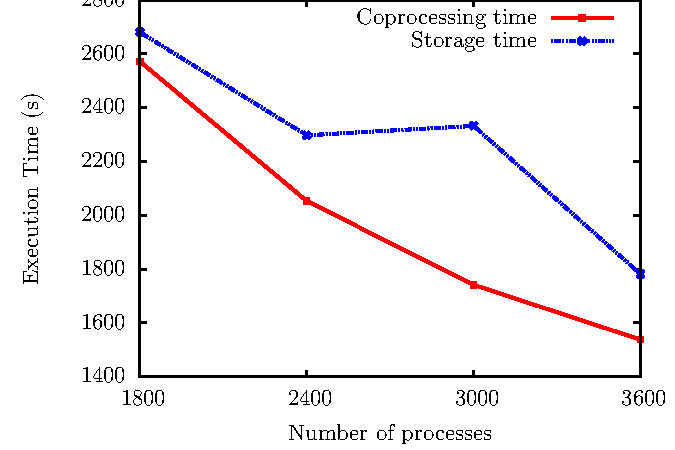
\includegraphics[scale=0.65]{pictures/test22.ps}
%\captionof{figure}{CASE\_B total execution time when using coprocessing and storage in
%Ensight Gold format.}
%\label{fig:204ensight}
%\vspace{+0.04in}
%~\
%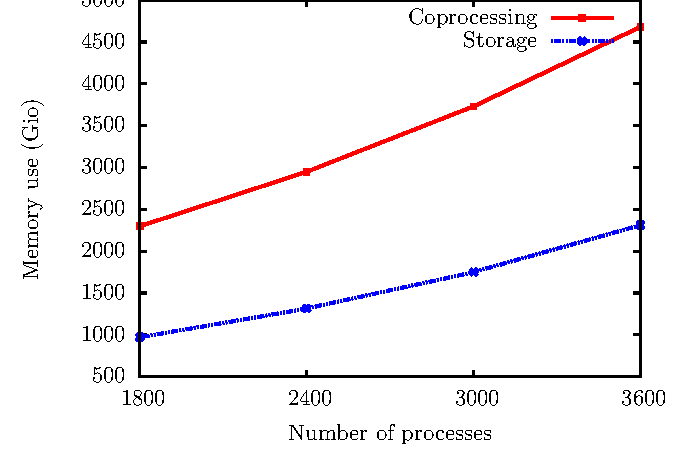
\includegraphics[scale=0.65]{pictures/test32.ps}
%\captionof{figure}{CASE\_B total memory usage when using coprocessing and storage in
%Ensight Gold format.}
%\label{fig:204mem}
%\end{minipage}
%\end{minipage}

        %\caption{CASE\_A results}\label{fig:animals}
%\end{figure}
%~
%\begin{figure}



%\clearpage


\section{Conclusion}
\label{sec:conclusion}

The main fact presented in this book chapter is that we have successfully
integrated Catalyst into \CS (a computational fluid dynamics code
developed at EDF R\&D). Both Catalyst and \CS are Open Source software
and this development can be download, used or tested freely by everyone. After
testing the prototype in our corporate supercomputer Ivanhoe, we find Catalyst to
be a relevant solution to provide \CS users with visualization
co-processing. Catalyst proved to allow a simple and fast implementation of an
adaptor.

The presented results are based on a 51M and a 204M elements mesh, which is
above the average size case used by EDF engineers in our industrial environment.
We plan to perform simulations on at least 400M elements meshes in the near
future, using the same supercomputer. We have also performed simulations up to
300 nodes and are currently planning not using more nodes. This is due to the
typical simulation node size in Ivanhoe being around 150 nodes for our
engineers. We also plan to work on another of our corporate supercomputers, an
IBM BG/Q with 65k cores. In that case, we will test on a much larger number of
cores.

The increase of memory use, described in the results section, indicates that
memory optimizations are to be performed before running on the IBM BG/Q. We did
not, in this study, perform any delicate memory tweaking in order to reduce the
memory consumption. We are currently working on this point, experimenting with
the new VTK in-situ data structures implemented recently by Kitware, the
so-called ``zero copy VTK''. This approach aims to facilitate the memory
management in the adaptor without the use of complicated pointer manipulation;
we expect to reduce memory overhead without much increasing code complexity.

Another ongoing development consists on how we deal with the ghost levels
generated by \CS. Indeed, we want to use the same spatial partition of
the meshes for \CS and Catalyst, the aim being not to degrade the
execution time by “not necessary data exchanges” among MPI ranks. We currently
use ParaView D3 filter (a filter originally performing a redistribution of the
data among MPI processes) as a ghost cell handler. However, we asked Kitware for
the integration in ParaView/Catalyst of a new filter to perform a direct
generation of ghost cells from existing distributed data. This development has
been finished in december 2013 before this book chapter is published.

This chapter has been dedicated on how to deal with large data using visual
co-processing but we are also testing the computational-steering capabilities of
Catalyst, the so-called Live Catalyst. This currently allows the modification of
the ParaView pipeline parameters while the numerical simulation is running.

In conclusion, we are mostly satisfied with the integration of Catalyst in
\CS. The first version of our integration will be released as part of a
new version of this open-source software.





%%%%%%%%%%%%%%%%%%%%%%%% referenc.tex %%%%%%%%%%%%%%%%%%%%%%%%%%%%%%
% sample references
% %
% Use this file as a template for your own input.
%
%%%%%%%%%%%%%%%%%%%%%%%% Springer-Verlag %%%%%%%%%%%%%%%%%%%%%%%%%%
%
% BibTeX users please use
% \bibliographystyle{}
% \bibliography{}
%
\biblstarthook{References may be \textit{cited} in the text either by number (preferred) or by author/year.\footnote{Make sure that all references from the list are cited in the text. Those not cited should be moved to a separate \textit{Further Reading} section or chapter.} The reference list should ideally be \textit{sorted} in alphabetical order -- even if reference numbers are used for the their citation in the text. If there are several works by the same author, the following order should be used: 
\begin{enumerate}
\item all works by the author alone, ordered chronologically by year of publication
\item all works by the author with a coauthor, ordered alphabetically by coauthor
\item all works by the author with several coauthors, ordered chronologically by year of publication.
\end{enumerate}
The \textit{styling} of references\footnote{Always use the standard abbreviation of a journal's name according to the ISSN \textit{List of Title Word Abbreviations}, see \url{http://www.issn.org/en/node/344}} depends on the subject of your book:
\begin{itemize}
\item The \textit{two} recommended styles for references in books on \textit{mathematical, physical, statistical and computer sciences} are depicted in ~\cite{science-contrib, science-online, science-mono, science-journal, science-DOI} and ~\cite{phys-online, phys-mono, phys-journal, phys-DOI, phys-contrib}.
\item Examples of the most commonly used reference style in books on \textit{Psychology, Social Sciences} are~\cite{psysoc-mono, psysoc-online,psysoc-journal, psysoc-contrib, psysoc-DOI}.
\item Examples for references in books on \textit{Humanities, Linguistics, Philosophy} are~\cite{humlinphil-journal, humlinphil-contrib, humlinphil-mono, humlinphil-online, humlinphil-DOI}.
\item Examples of the basic Springer style used in publications on a wide range of subjects such as \textit{Computer Science, Economics, Engineering, Geosciences, Life Sciences, Medicine, Biomedicine} are ~\cite{basic-contrib, basic-online, basic-journal, basic-DOI, basic-mono}. 
\end{itemize}
}

\begin{thebibliography}{99.}%
% and use \bibitem to create references.
%
% Use the following syntax and markup for your references if 
% the subject of your book is from the field 
% "Mathematics, Physics, Statistics, Computer Science"
%
% Contribution 
\bibitem{science-contrib} Broy, M.: Software engineering --- from auxiliary to key technologies. In: Broy, M., Dener, E. (eds.) Software Pioneers, pp. 10-13. Springer, Heidelberg (2002)
%
% Online Document
\bibitem{science-online} Dod, J.: Effective substances. In: The Dictionary of Substances and Their Effects. Royal Society of Chemistry (1999) Available via DIALOG. \\
\url{http://www.rsc.org/dose/title of subordinate document. Cited 15 Jan 1999}
%
% Monograph
\bibitem{science-mono} Geddes, K.O., Czapor, S.R., Labahn, G.: Algorithms for Computer Algebra. Kluwer, Boston (1992) 
%
% Journal article
\bibitem{science-journal} Hamburger, C.: Quasimonotonicity, regularity and duality for nonlinear systems of partial differential equations. Ann. Mat. Pura. Appl. \textbf{169}, 321--354 (1995)
%
% Journal article by DOI
\bibitem{science-DOI} Slifka, M.K., Whitton, J.L.: Clinical implications of dysregulated cytokine production. J. Mol. Med. (2000) doi: 10.1007/s001090000086 
%
\bigskip

% Use the following (APS) syntax and markup for your references if 
% the subject of your book is from the field 
% "Mathematics, Physics, Statistics, Computer Science"
%
% Online Document
\bibitem{phys-online} J. Dod, in \textit{The Dictionary of Substances and Their Effects}, Royal Society of Chemistry. (Available via DIALOG, 1999), 
\url{http://www.rsc.org/dose/title of subordinate document. Cited 15 Jan 1999}
%
% Monograph
\bibitem{phys-mono} H. Ibach, H. L\"uth, \textit{Solid-State Physics}, 2nd edn. (Springer, New York, 1996), pp. 45-56 
%
% Journal article
\bibitem{phys-journal} S. Preuss, A. Demchuk Jr., M. Stuke, Appl. Phys. A \textbf{61}
%
% Journal article by DOI
\bibitem{phys-DOI} M.K. Slifka, J.L. Whitton, J. Mol. Med., doi: 10.1007/s001090000086
%
% Contribution 
\bibitem{phys-contrib} S.E. Smith, in \textit{Neuromuscular Junction}, ed. by E. Zaimis. Handbook of Experimental Pharmacology, vol 42 (Springer, Heidelberg, 1976), p. 593
%
\bigskip
%
% Use the following syntax and markup for your references if 
% the subject of your book is from the field 
% "Psychology, Social Sciences"
%
%
% Monograph
\bibitem{psysoc-mono} Calfee, R.~C., \& Valencia, R.~R. (1991). \textit{APA guide to preparing manuscripts for journal publication.} Washington, DC: American Psychological Association.
%
% Online Document
\bibitem{psysoc-online} Dod, J. (1999). Effective substances. In: The dictionary of substances and their effects. Royal Society of Chemistry. Available via DIALOG. \\
\url{http://www.rsc.org/dose/Effective substances.} Cited 15 Jan 1999.
%
% Journal article
\bibitem{psysoc-journal} Harris, M., Karper, E., Stacks, G., Hoffman, D., DeNiro, R., Cruz, P., et al. (2001). Writing labs and the Hollywood connection. \textit{J Film} Writing, 44(3), 213--245.
%
% Contribution 
\bibitem{psysoc-contrib} O'Neil, J.~M., \& Egan, J. (1992). Men's and women's gender role journeys: Metaphor for healing, transition, and transformation. In B.~R. Wainrig (Ed.), \textit{Gender issues across the life cycle} (pp. 107--123). New York: Springer.
%
% Journal article by DOI
\bibitem{psysoc-DOI}Kreger, M., Brindis, C.D., Manuel, D.M., Sassoubre, L. (2007). Lessons learned in systems change initiatives: benchmarks and indicators. \textit{American Journal of Community Psychology}, doi: 10.1007/s10464-007-9108-14.
%
%
% Use the following syntax and markup for your references if 
% the subject of your book is from the field 
% "Humanities, Linguistics, Philosophy"
%
\bigskip
%
% Journal article
\bibitem{humlinphil-journal} Alber John, Daniel C. O'Connell, and Sabine Kowal. 2002. Personal perspective in TV interviews. \textit{Pragmatics} 12:257--271
%
% Contribution 
\bibitem{humlinphil-contrib} Cameron, Deborah. 1997. Theoretical debates in feminist linguistics: Questions of sex and gender. In \textit{Gender and discourse}, ed. Ruth Wodak, 99--119. London: Sage Publications.
%
% Monograph
\bibitem{humlinphil-mono} Cameron, Deborah. 1985. \textit{Feminism and linguistic theory.} New York: St. Martin's Press.
%
% Online Document
\bibitem{humlinphil-online} Dod, Jake. 1999. Effective substances. In: The dictionary of substances and their effects. Royal Society of Chemistry. Available via DIALOG. \\
http://www.rsc.org/dose/title of subordinate document. Cited 15 Jan 1999
%
% Journal article by DOI
\bibitem{humlinphil-DOI} Suleiman, Camelia, Daniel C. O and Sabine Kowal. 2002. `If you and I, if we, in this later day, lose that sacred fire...': Perspective in political interviews. \textit{Journal of Psycholinguistic Research}. doi: 10.1023/A:1015592129296.
%
%
%
\bigskip
%
%
% Use the following syntax and markup for your references if 
% the subject of your book is from the field 
% "Computer Science, Economics, Engineering, Geosciences, Life Sciences"
%
%
% Contribution 
\bibitem{basic-contrib} Brown B, Aaron M (2001) The politics of nature. In: Smith J (ed) The rise of modern genomics, 3rd edn. Wiley, New York 
%
% Online Document
\bibitem{basic-online} Dod J (1999) Effective Substances. In: The dictionary of substances and their effects. Royal Society of Chemistry. Available via DIALOG. \\
\url{http://www.rsc.org/dose/title of subordinate document. Cited 15 Jan 1999}
%
% Journal article by DOI
\bibitem{basic-DOI} Slifka MK, Whitton JL (2000) Clinical implications of dysregulated cytokine production. J Mol Med, doi: 10.1007/s001090000086
%
% Journal article
\bibitem{basic-journal} Smith J, Jones M Jr, Houghton L et al (1999) Future of health insurance. N Engl J Med 965:325--329
%
% Monograph
\bibitem{basic-mono} South J, Blass B (2001) The future of modern genomics. Blackwell, London 
%
\end{thebibliography}

\end{document}
